\documentclass[]{article}
\usepackage{lmodern}
\usepackage{amssymb,amsmath}
\usepackage{ifxetex,ifluatex}
\usepackage{fixltx2e} % provides \textsubscript
\ifnum 0\ifxetex 1\fi\ifluatex 1\fi=0 % if pdftex
  \usepackage[T1]{fontenc}
  \usepackage[utf8]{inputenc}
\else % if luatex or xelatex
  \ifxetex
    \usepackage{mathspec}
  \else
    \usepackage{fontspec}
  \fi
  \defaultfontfeatures{Ligatures=TeX,Scale=MatchLowercase}
\fi
% use upquote if available, for straight quotes in verbatim environments
\IfFileExists{upquote.sty}{\usepackage{upquote}}{}
% use microtype if available
\IfFileExists{microtype.sty}{%
\usepackage[]{microtype}
\UseMicrotypeSet[protrusion]{basicmath} % disable protrusion for tt fonts
}{}
\PassOptionsToPackage{hyphens}{url} % url is loaded by hyperref
\usepackage[unicode=true]{hyperref}
\hypersetup{
            pdftitle={Results},
            pdfborder={0 0 0},
            breaklinks=true}
\urlstyle{same}  % don't use monospace font for urls
\usepackage[margin=1in]{geometry}
\usepackage{graphicx,grffile}
\makeatletter
\def\maxwidth{\ifdim\Gin@nat@width>\linewidth\linewidth\else\Gin@nat@width\fi}
\def\maxheight{\ifdim\Gin@nat@height>\textheight\textheight\else\Gin@nat@height\fi}
\makeatother
% Scale images if necessary, so that they will not overflow the page
% margins by default, and it is still possible to overwrite the defaults
% using explicit options in \includegraphics[width, height, ...]{}
\setkeys{Gin}{width=\maxwidth,height=\maxheight,keepaspectratio}
\IfFileExists{parskip.sty}{%
\usepackage{parskip}
}{% else
\setlength{\parindent}{0pt}
\setlength{\parskip}{6pt plus 2pt minus 1pt}
}
\setlength{\emergencystretch}{3em}  % prevent overfull lines
\providecommand{\tightlist}{%
  \setlength{\itemsep}{0pt}\setlength{\parskip}{0pt}}
\setcounter{secnumdepth}{0}
% Redefines (sub)paragraphs to behave more like sections
\ifx\paragraph\undefined\else
\let\oldparagraph\paragraph
\renewcommand{\paragraph}[1]{\oldparagraph{#1}\mbox{}}
\fi
\ifx\subparagraph\undefined\else
\let\oldsubparagraph\subparagraph
\renewcommand{\subparagraph}[1]{\oldsubparagraph{#1}\mbox{}}
\fi

% set default figure placement to htbp
\makeatletter
\def\fps@figure{htbp}
\makeatother

\usepackage{booktabs}
\usepackage{longtable}
\usepackage{array}
\usepackage{multirow}
\usepackage{wrapfig}
\usepackage{float}
\usepackage{colortbl}
\usepackage{pdflscape}
\usepackage{tabu}
\usepackage{threeparttable}
\usepackage{threeparttablex}
\usepackage[normalem]{ulem}
\usepackage{makecell}
\usepackage{xcolor}

\title{Results}
\author{}
\date{\vspace{-2.5em}}

\begin{document}
\maketitle

An introduction to results. A description of each one of the results.

\subsubsection{Participants}\label{participants}

\begin{table}

\caption{\label{tab:unnamed-chunk-1}Participants demographics}
\centering
\begin{tabular}[t]{l|l|l|l|l|l|l|l|l|l}
\hline
participant & gender & age & occupation & country of origin & type accomodation & people in accomodation & inhabitants in accomodation & first session & helpers\\
\hline
\rowcolor{gray!6}  1 & male & 25 & PhD student & Indonesia & house & 2 & professionals & reg & -\\
\hline
2 & non binary & 28 & PhD student & Germany & house & 4 & students & new & -\\
\hline
\rowcolor{gray!6}  3 & male & 19 & Undergraduate student & Hong Kong & flat & 6 & students & reg & -\\
\hline
4 & female & 50 & Impact officer & USA & house & 4 & family & new & -\\
\hline
\rowcolor{gray!6}  5 & male & 30 & Administrator & UK & house & 2 & couple & reg & new\\
\hline
6 & female & 32 & Jobseeker & Hong Kong & house & 4 & professionals & reg & -\\
\hline
\rowcolor{gray!6}  7 & male & 32 & PhD student & Iraq & flat & 3 & family & reg & -\\
\hline
8 & female & 33 & PhD student & Russia & flat & 1 & individual & reg & -\\
\hline
\rowcolor{gray!6}  9 & female & 29 & Invigilator & Mexico & flat & 2 & couple & new & reg \& new\\
\hline
10 & male & 29 & PhD student & Greece & flat & 2 & couple & reg & -\\
\hline
\rowcolor{gray!6}  11 & female & 29 & PhD student & Bosnia and Herzegovina & flat & 2 & couple & new & -\\
\hline
12 & male & 46 & Researcher & Mexico & house & 5 & family & reg & -\\
\hline
\rowcolor{gray!6}  13 & female & 29 & Lecturer & UK & house & 2 & couple & new & new\\
\hline
14 & female & 35 & Housewife & Mexico & house & 4 & family & new & -\\
\hline
\rowcolor{gray!6}  15 & female & 72 & Retired & Puerto Rico & house & 2 & couple & new & -\\
\hline
16 & female & 40 & Housewife & Mexico & house & 3 & family & reg & -\\
\hline
\rowcolor{gray!6}  17 & female & 32 & Research fellow & Ireland & house & 6 & professionals & reg & -\\
\hline
18 & female & 26 & Food scientist & UK & house & 3 & professionals & new & reg \& new\\
\hline
\rowcolor{gray!6}  19 & female & 37 & Supply chain manager & China & house & 3 & family & new & -\\
\hline
20 & female & 46 & School director & UK & house & 3 & family & reg & -\\
\hline
\end{tabular}
\end{table}

\subsubsection{Recipes}\label{recipes}

Add recipe source

\begin{table}

\caption{\label{tab:unnamed-chunk-2}List of recipes}
\centering
\begin{tabular}[t]{l|l|l}
\hline
session & regular & new\\
\hline
\rowcolor{gray!6}  1 & chicken coconut curry & mac and cheese\\
\hline
2 & chickpeas curry with rice & butternut squash curry with coconut milk\\
\hline
\rowcolor{gray!6}  3 & pasta bolognesa & stir fry chicken, rice and peas\\
\hline
4 & green vegs soup & creamy tomato and chorizo rigatoni\\
\hline
\rowcolor{gray!6}  5 & pasta bolognesa & mexican chicken stew\\
\hline
6 & noddles with vegetables (spaggetti) & chicken gyros\\
\hline
\rowcolor{gray!6}  7 & oven roasted chicken & pomegranate rice and salad\\
\hline
8 & scrambled eggs with vegs & ricotta pancakes\\
\hline
\rowcolor{gray!6}  9 & chicken fajitas with rice and fried beans & beef, bean, and beer chili\\
\hline
10 & scrambled eggs with vegs and sausages & mushroom risotto\\
\hline
\rowcolor{gray!6}  11 & pasta bolognesa with vegs & crispy five-spice chicken\\
\hline
12 & minced vegs with vegetables tacos & spanish tortilla (potatoes omelette)\\
\hline
\rowcolor{gray!6}  13 & creamy risssoto with vegs and prawns & keralan chicken curry\\
\hline
14 & vegetable-based stew & cream of spinach soup\\
\hline
\rowcolor{gray!6}  15 & rice with chickpeas (puerto rican rice) & spinach and chickpea soup\\
\hline
16 & roasted chicken and roasted vegetables & white beans with artichokes\\
\hline
\rowcolor{gray!6}  17 & shepherd's pie & szechuan cabbage and crispy chilli beef\\
\hline
18 & pasta carbonara \& pasta napolitana & malfatti ricotta and spinach \& hummus\\
\hline
\rowcolor{gray!6}  19 & shepherd's pie & prawn and black beans curry\\
\hline
20 & creamy chicken pasta & spicy beef with coriander relish\\
\hline
\end{tabular}
\end{table}

\subsubsection{Inventory CPGs}\label{inventory-cpgs}

\begin{table}

\caption{\label{tab:unnamed-chunk-3}Inventory CPGs}
\centering
\begin{tabular}[t]{l|l}
\hline
participant & number of CPGs\\
\hline
\rowcolor{gray!6}  1 & 121\\
\hline
2 & 199\\
\hline
\rowcolor{gray!6}  3 & 38\\
\hline
4 & 158\\
\hline
\rowcolor{gray!6}  5 & 266\\
\hline
6 & 204\\
\hline
\rowcolor{gray!6}  7 & 155\\
\hline
8 & 220\\
\hline
\rowcolor{gray!6}  9 & 196\\
\hline
10 & 138\\
\hline
\rowcolor{gray!6}  11 & 208\\
\hline
12 & 206\\
\hline
\rowcolor{gray!6}  13 & 179\\
\hline
14 & 301\\
\hline
\rowcolor{gray!6}  15 & 254\\
\hline
16 & 212\\
\hline
\rowcolor{gray!6}  17 & 423\\
\hline
18 & 99\\
\hline
\rowcolor{gray!6}  19 & 189\\
\hline
20 & 272\\
\hline
\end{tabular}
\end{table}

\subsubsection{Duration recipes}\label{duration-recipes}

\begin{table}

\caption{\label{tab:unnamed-chunk-4}Duration of recipes}
\centering
\begin{tabular}[t]{l|l|l}
\hline
session & regular & new\\
\hline
\rowcolor{gray!6}  1 & 36 & 61\\
\hline
2 & 76 & 81\\
\hline
\rowcolor{gray!6}  3 & 21 & 40\\
\hline
4 & 45 & 52\\
\hline
\rowcolor{gray!6}  5 & 41 & 90\\
\hline
6 & 45 & 90\\
\hline
\rowcolor{gray!6}  7 & 88 & 29\\
\hline
8 & 28 & 34\\
\hline
\rowcolor{gray!6}  9 & 68 & 78\\
\hline
10 & 39 & 111\\
\hline
\rowcolor{gray!6}  11 & 56 & 87\\
\hline
12 & 80 & 126\\
\hline
\rowcolor{gray!6}  13 & 42 & 53\\
\hline
14 & 73 & 58\\
\hline
\rowcolor{gray!6}  15 & 50 & 46\\
\hline
16 & 70 & 47\\
\hline
\rowcolor{gray!6}  17 & 113 & 90\\
\hline
18 & 44 & 80\\
\hline
\rowcolor{gray!6}  19 & 70 & 61\\
\hline
20 & 68 & 17\\
\hline
\end{tabular}
\end{table}

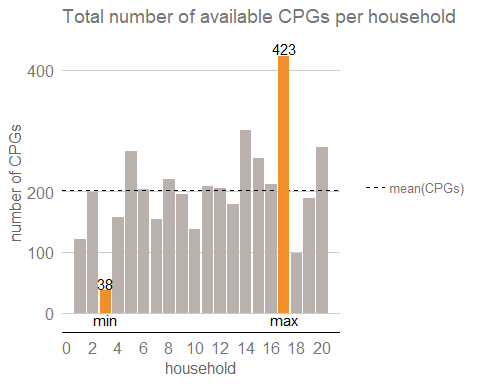
\includegraphics{test_files/figure-latex/unnamed-chunk-5-1.pdf}

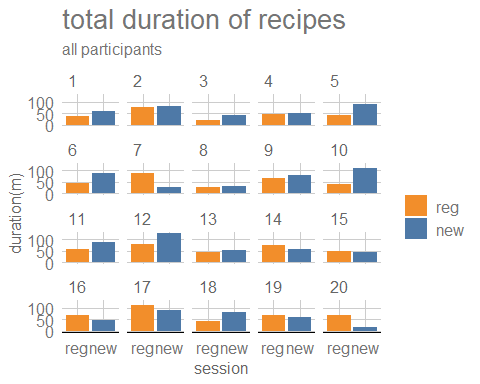
\includegraphics{test_files/figure-latex/unnamed-chunk-6-1.pdf}

\subsubsection{Items used}\label{items-used}

The list of the items used

\begin{table}

\caption{\label{tab:unnamed-chunk-7}Total number of different items used}
\centering
\begin{tabular}[t]{c|c|c|c|c}
\hline
session & c & u & e & total\\
\hline
all & 970 & 1308 & 496 & 2774\\
\hline
regular & 465 & 567 & 237 & 1269\\
\hline
new & 505 & 741 & 259 & 1505\\
\hline
\multicolumn{5}{l}{\textsuperscript{*} c = CPGs, u = utensil, e = environment}\\
\end{tabular}
\end{table}

\subsubsection{Total number of different items
used}\label{total-number-of-different-items-used}

The total number of different items used were as follows:

\begin{table}

\caption{\label{tab:unnamed-chunk-8}Total number of different items used}
\centering
\begin{tabular}[t]{c|c|c|c|c}
\hline
session & c & u & e & total\\
\hline
all & 970 & 1308 & 496 & 2774\\
\hline
regular & 465 & 567 & 237 & 1269\\
\hline
new & 505 & 741 & 259 & 1505\\
\hline
\multicolumn{5}{l}{\textsuperscript{*} c = CPGs, u = utensil, e = environment}\\
\end{tabular}
\end{table}

id

unique

subcategory

id

unique

subcategory

id

unique

subcategory

1

alioli

condiment

26

cardamon

spice

51

coriander

veg

2

alumFoil

disposableCover

27

caribeanSpices

spice

52

corianderPwd

spice

3

artichoke

veg

28

carrots

veg

53

corn

preparedCarbs

4

asparagus

veg

29

cayenne

spice

54

cornFlour

textureModifier

5

aubergine

veg

30

celery

veg

55

courgette

veg

6

avocado

veg

31

cheese

dairy

56

cream

dairy

7

bacon

meat

32

chicken

meat

57

cucumber

veg

8

bag

disposableCover

33

chickpeas

preparedCarbs

58

cumin

spice

9

bagFreezer

disposableCover

34

chillies

veg

59

curry

spice

10

bakingPaper

disposableCover

35

chilliesFlakes

spice

60

disposables

disposableCover

11

bakingPwd

textureModifier

36

chilliesPwd

spice

61

dWashL

cleaningProduct

12

basil

veg

37

chineseGreens

veg

62

eggs

meat

13

basilPwd

spice

38

chineseSpice

spice

63

fennel

spice

14

beans

preparedCarbs

39

chips

preparedCarbs

64

fishSauce

condiment

15

beanSprouts

veg

40

chives

spice

65

fiveSpicesSeasoning

spice

16

beef

meat

41

chorizo

meat

66

flour

textureModifier

17

beer

beverage

42

cider

beverage

67

food

food

18

bellPepper

veg

43

cilantroBase

condiment

68

frozenVegs

veg

19

blackPepper

spice

44

cinamon

spice

69

garlic

veg

20

bouillon

spice

45

cleaningLiquid

cleaningProducts

70

garlicPwd

spice

21

bread

preparedCarbs

46

clingFilm

disposableCover

71

ginger

veg

22

butter

dairy

47

cloth

cleaningProducts

72

gloves

cleaningProducts

23

butternutSquash

veg

48

cocoa

spice

73

goyaSeasoning

spice

24

cabbage

veg

49

coconutCream

condiment

74

greenBeans

veg

25

cake

preparedCarbs

50

coffee

beverage

75

greenSnaps

veg

\subsection{Including Plots}\label{including-plots}

You can also embed plots, for example:

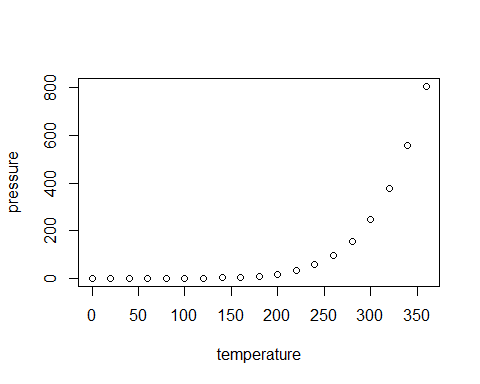
\includegraphics{test_files/figure-latex/pressure-1.pdf}

Note that the \texttt{echo\ =\ FALSE} parameter was added to the code
chunk to prevent printing of the R code that generated the plot

\end{document}
